\documentclass[a4paper,10pt]{article}
\usepackage[utf8]{inputenc}
\usepackage{amsfonts}
\usepackage{amssymb}
\usepackage{amsmath}
\usepackage{amsbsy}
\usepackage{ragged2e}
\usepackage{graphicx}
\usepackage[verbose]{wrapfig}
\usepackage{changepage}
\usepackage{float}
\usepackage{cite}
\usepackage{url}
\usepackage{geometry}                         
\geometry{left=18mm,right=18mm,top=21mm,bottom=21mm}
\usepackage[spanish]{babel}
\usepackage[usenames,dvipsnames]{xcolor}
\pagecolor{white}
\usepackage{multirow}
\definecolor{wiki}{rgb}{1,0.5,0}
\usepackage{tikz}
\usepackage{array}
\usepackage[all]{xy}
\usepackage{tabularx}
\usepackage{subcaption}
\graphicspath{Images}
\pagestyle{plain} 
\pagenumbering{arabic}
\usepackage{lastpage}
\usepackage{fancyhdr}
\pagestyle{fancy}
\usepackage{lipsum}
\usepackage{booktabs}
\usepackage{skull}
\usepackage{multicol}
\usepackage{parcolumns}
\usepackage{soul}
\usepackage[hidelinks]{hyperref} 


\definecolor{MiColor1}{RGB}{135,2,1}
\definecolor{MiColor2}{RGB}{254,80,0}
\definecolor{MiColor3}{RGB}{44,135,240}
\definecolor{MiColor4}{RGB}{6,69,173}
\definecolor{MiColor5}{RGB}{51,102,187}

\lhead{\protect\href{https://www.uaeh.edu.mx/}{
\includegraphics[width=.12\textwidth]{Images/UAEH Logo.png}}} 
\chead{\itshape{Agosto 2020}}
\rhead{\colorbox{MiColor1}{\textcolor{White}{\protect\href{https://www.uaeh.edu.mx/campus/icbi/oferta/licenciaturas/lic_fisica.html}{LiFTA}}}} 
\lfoot{} 
\cfoot{\thepage\ de \pageref{LastPage}} 
\rfoot{}


\renewcommand{\headrulewidth}{2pt}
\renewcommand{\footrulewidth}{0pt}



\setlength\headheight{55.0pt}
\addtolength{\textheight}{-40.0pt}
%-------------------------------%

\newcounter{resumen}
\setcounter{resumen}{0}
\def\theejemplo{\thechapter.\arabic{resumen}}

\newenvironment{resumen}
{	\begin{center}
	\begin{minipage}[t!]{480 pt}
	\vspace{2mm}
	\emph{\textcolor{MiColor1}{\textbf{Resumen}}}
	\\[-1mm]
	\\[-10mm]
	\hfill 
	   \begin{wrapfigure}{hbt!}{5.3cm}
       \centering
       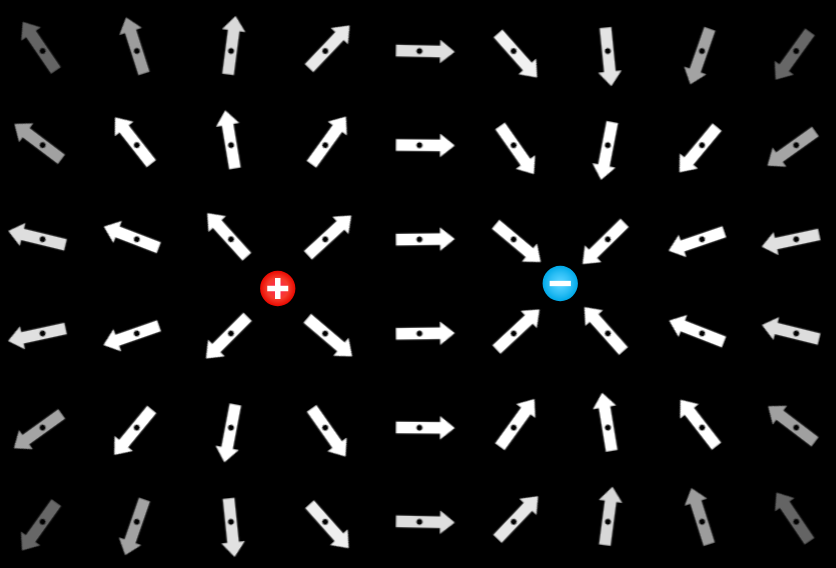
\includegraphics[scale=0.3]{Images/Cargas y Campos.PNG}
       \end{wrapfigure} \vspace{-4mm}
    \hfill
	\textcolor{Black}{\line(1,0){480}}\\ \par
}
{
	\par \normalsize \par
	\par \\[3mm] \par
	\vspace{4mm}
	\par \footnotesize\textbf{Palabras clave: \footnotesize\@palabras}
	\\[-1mm]
	\textcolor{Black}{\line(1,0){480}}\\ \par
	\\[5cm]
	\end{minipage}
	\vspace{0.5cm}
	\end{center}
}


\def\palabras#1{\gdef\@palabras{#1}}

\palabras{Cargas Eléctricas, Campo vectorial, Atracción, Repulsión, Lineas de campo eléctrico, Distancia, Potencial y Simulación.} 

%-------------------------------%

\begin{document}

{\textbf{\LARGE Mapeo de Cargas Eléctricas} \par} \vspace{3mm}
{\small A. D. Hernández-Melo\textcolor{Plum}{$^\heartsuit$}, E. S. Pulido-Reyes\textcolor{ProcessBlue}{$^\diamondsuit$}, y A. A. Santoyo-Noeggerath\textcolor{Green}{$^\dagger$} \par} \vspace{3mm}
{\footnotesize \textcolor{Plum}{$^\heartsuit$}\textcolor{ProcessBlue}{$^\diamondsuit$}\textcolor{Green}{$^\dagger$}\protect\href{https://www.google.com/maps/place/\%C3\%81rea+Acad\%C3\%A9mica+de+Matem\%C3\%A1ticas+y+F\%C3\%ADsica,+Universidad+Aut\%C3\%B3noma+del+Estado+de+Hidalgo,+Universidad+Autonoma+del+Estado+de+Hidalgo/@20.0934375,-98.7104375,17z/data=!4m13!1m7!3m6!1s0x0:0x0!2s76G337VQ\%2B9R!3b1!8m2!3d20.0934375!4d-98.7104375!3m4!1s0x85d1a773691bc455:0xe552799fa3ca76a5!8m2!3d20.0933901!4d-98.7104677}{Área Académica de Matemáticas y Física, Instituto de Ciencias Básicas e Ingenierías, Universidad Autónoma del Estado} \par} 
{\footnotesize \protect\href{https://www.google.com/maps/place/\%C3\%81rea+Acad\%C3\%A9mica+de+Matem\%C3\%A1ticas+y+F\%C3\%ADsica,+Universidad+Aut\%C3\%B3noma+del+Estado+de+Hidalgo,+Universidad+Autonoma+del+Estado+de+Hidalgo/@20.0934375,-98.7104375,17z/data=!4m13!1m7!3m6!1s0x0:0x0!2s76G337VQ\%2B9R!3b1!8m2!3d20.0934375!4d-98.7104375!3m4!1s0x85d1a773691bc455:0xe552799fa3ca76a5!8m2!3d20.0933901!4d-98.7104677}{de Hidalgo, Carretera Pachuca-Tulancingo Km. 4.5, Col. Carboneras, C.P. 42184, Mineral de la Reforma, Hidalgo, México} \par}
{\footnotesize \textit{Contacto}: \textcolor{Plum}{$^\heartsuit$}\protect\href{mailto:he312453@uaeh.edu.mx}{he312453@uaeh.edu.mx},  \textcolor{ProcessBlue}{$^\diamondsuit$}\protect\href{mailto:pu359528@uaeh.edu.mx}{pu359528@uaeh.edu.mx}, \textcolor{Green}{$^\dagger$}\protect\href{mailto:sa352740@uaeh.edu.mx}{sa352740@uaeh.edu.mx}}

\begin{resumen}
Con apoyo del software \textit{PhET} vamos a observar como se comportan las lineas de campo eléctrico cuando hay una o más cargas de signo igual o diferente (esto se puede cambiar a elección), se experimentará metiendo cargas y aumentando las magnitudes de la misma intentando apilar cargas de los valores $1$ y $-1 nC$ (nano coulomb) o simplemente realizando diferentes sistemas para los diferentes cálculos que se planteen, se podrá medir el equipotencial total en los diferentes puntos del sistema (ya sea pegado a la carga o a algunos centímetros ($cm$) o metros ($m$)  de distancia) así como en diferentes casos  y con ayuda de un pequeño metro virtual sera posible medir la distancia entre las cargas, ya sea para poder comprobar los cálculos respecto al equipotencial (con ayuda del campo eléctrico), crear nuestros propios cálculos o para replicar algún sistema visto en un problema, etc. Todo esto para tener un sustento experimental y más gráfico de lo visto durante las clases del curso de Electromagnetismo.
\end{resumen}

\begin{multicols}{2}
\section{\textcolor{MiColor1}{\textbf{Introducción}}}
El objetivo con el que se realizó esta práctica es poder comprender los patrones que generan los campos eléctricos, que si bien, las analizamos en primera instancia en espacios bidimensionales, podemos trasladarlas a un espacio tridimensional (utilizando herramientas matemáticas como los campos vectoriales). Primero partimos de la definición de un campo eléctrico, que en su representación matemática sería:\par
    \vspace{2mm}
    \centerline{$\Vec{E}=\dfrac{\Vec{F}_0}{q_0}$} \par
El \textit{campo eléctrico} $\Vec{E}$ en un punto se define como la fuerza eléctrica $\Vec{F}_0$ que experimenta una carga de prueba $q_0$ en dicho punto, dividida entre la carga $q_0$. (H. D. Young, R. A. Freedman. 2013)\cite{2}. \\
Que, reescribiendo la ecuación anterior, haciendo uso de la ley de Coulomb tenemos que:\par
    \vspace{2mm}
    \centerline{$\Vec{F}=\dfrac{1}{4\pi{\epsilon}_0}\dfrac{|qq_0|}{r^2}\Vec{r}$\hspace{1em};\hspace{1em}(Ley de Coulomb)}\par
    \vspace{1em}
    \centerline{$\Vec{E}=\dfrac{1}{4\pi{\epsilon}_0}\dfrac{q}{r^2}\hat{r}$}\par
    \vspace{2mm}
Cabe aclarar que el caso anterior es para \textbf{cargas puntuales}. Ahora bien, en la realidad no puede apreciarse un campo eléctrico directamente, por lo que, para visualizarlos hacemos uso de las \textbf{líneas de campo eléctrico}, que podemos describirlas como líneas o curvas imaginarias que se distribuyen de manera radial alrededor de una carga puntual, que dependiendo del valor de la carga se dirigirán hacia afuera de la carga ($+q$) o hacia adentro de la carga ($-q$).\\
El número de líneas por unidad de área que pasan a través de una superficie perpendicular a dichas líneas es proporcional a la magnitud del campo eléctrico en
dicha región. En consecuencia, las líneas de campo estarán cercanas donde el campo
eléctrico sea intenso y separadas donde el campo sea débil. (R. Serway, J. Jewett. 2009)\cite{1}.\par
Sabemos que en cuanto a fuerzas eléctricas se refiere, tenemos una fuerza de repulsión o atracción, que dependiendo del valor de las cargas de un sistema será una u otra. Un caso sencillo de una fuerza de atracción son los dipolos eléctricos, pues bien, la cantidad de las líneas de campo que surgirían de la carga positiva serían iguales a la cantidad que terminarían en la carga negativa. Entre ambas cargas se originaría una densidad de líneas que indicarían una región en la cual indicaría que el campo eléctrico es intenso.
Pero, en el caso en el que ambas cargas fuesen iguales ($+q$), es decir que originen una fuerza de repulsión, ambas cargas generarían la misma cantidad de líneas de campo y a una distancia considerable de las cargas, el campo eléctrico es similar al valor de una sola carga puntual de magnitud $2q$. \\
Es preciso mencionar que las líneas de campo nunca se cruzan, esto se debe a que un campo eléctrico no puede tener dos direcciones distintas en un punto dado, ni ejercer más fuerza sobre una carga de prueba. \cite{8} \par
También, utilizamos el concepto de \textbf{potencial eléctrico}, para calcular el voltaje que generan las diferentes cargas que fueron simuladas, la expresión matemática más sencilla para calcular el voltaje de una carga viene dado por: \par
\vspace{2mm}
\centerline{$V=\dfrac{U}{q_0}$}\par
\vspace{2mm}
Para el caso del \textit{diferencial de potencial eléctrico} usamos la expresión:\par
\vspace{2mm}
\centerline{$\Delta V=\dfrac{\Delta U}{q_0}=- \displaystyle\int_{\tiny \textcircled{a}}^{\tiny \textcircled{b}}\Vec{E}\cdot d\Vec{s}$} \par
\vspace{2mm}
Donde {\small \textcircled{a}} y {\small \textcircled{b}} son las posiciones en las que se desplaza la carga, y $d\Vec{s}$ para indicar un vector de desplazamiento infinitesimal. \cite{1} \par
Todas estas cuestiones del campo eléctrico y líneas de campo en algún punto fueron explicadas por \textit{Faraday}, que en su momento utilizaría recursos propios de aquel entonces. Hoy en día contamos con más de una técnica para poder explicar de manera experimental los campos eléctricos y las líneas de campo, en este documento hacemos uso de una extensión web\cite{5} (proporcionada por la \textit{University of Colorado Boulder}). \par

\section{\textcolor{MiColor1}{\textbf{Materiales y Desarrollo Experimental}}}

\begin{table}[H]
    \centering
    \begin{tabular}{||>{\centering\arraybackslash}m{3.5cm} |>{\centering\arraybackslash}m{3.5cm}||}
    \hline
       \multirow{2}{3.5cm}{\centering\textbf{Descripción}} & \multirow{2}{3.5cm}{\centering\textbf{Especificaciones}} \\
        &  \\
    \hline \hline
       \multirow{3}{3.5cm}{\centering Ordenador Convencional} & \multirow{3}{3.5cm}{\centering Conexión a Internet} \\
        &  \\
        &  \\
    \hline
       \multirow{4}{3.5cm}{\centering Software (Ordenador)} & \multirow{4}{3.5cm}{\centering Extensión Web \textit{PhET: Interactive Simulations}\cite{5}} \\
        &  \\
        &  \\
        &  \\
    \hline
       \multirow{2}{3.5cm}{\centering Software (Ordenador)} & \multirow{2}{3.5cm}{\centering OriginPro 2019} \\
        &  \\
    \hline
    \end{tabular}
\end{table}
\vspace{-3mm}
\begin{center}
    \textbf{Tabla de Materiales}
\end{center}
\vspace{-3mm}
\subsection{\textcolor{MiColor1}{\textbf{Métodos Experimentales}}}
Dentro del simulador \textit{PhET} y con ayuda de él como herramienta principal para la experimentación en esta práctica, se colocó una carga positiva al centro del área de prueba, posteriormente se midió el voltaje con la herramienta \textit{Equipotencial} a distintos radios de la partícula en cuestión registrando los vectores en distintas posiciones del plano de trabajo a distintas distancias de la carga incluyendo las pociones sobre la carga respectivamente. En seguida se retiró la carga positiva suplantándola por la carga negativa repitiendo el procedimiento. Para proceder se colocará una sola carga (positiva) y se variará la distancia a un punto cualquiera $P$ para observar el comportamiento del campo eléctrico y la relación que tiene con el equipotencial en dicha distancia (la misma distancia a la que se calculará el campo eléctrico, será la distancia a la que se va a comparar con el equipotencial), para la parte de equipotencial se utilizara la herramienta incluida con el software, posteriormente se añadirá una carga de signo opuesto (en este caso signo negativo) a $6.1$ metros ($m$) de distancia de la carga que se coloco anteriormente para observar lo que ocurre y como cambian los valores obtenidos (con las mismas distancias que anteriormente manejamos) y para finalizar se comparara la relación que tienen el campo eléctrico, la carga eléctrica y si estas dos guardan alguna relación con el equipotencial. \vspace{-1cm}
\section{\textcolor{MiColor1}{\textbf{Resultados}}}

\begin{center}
      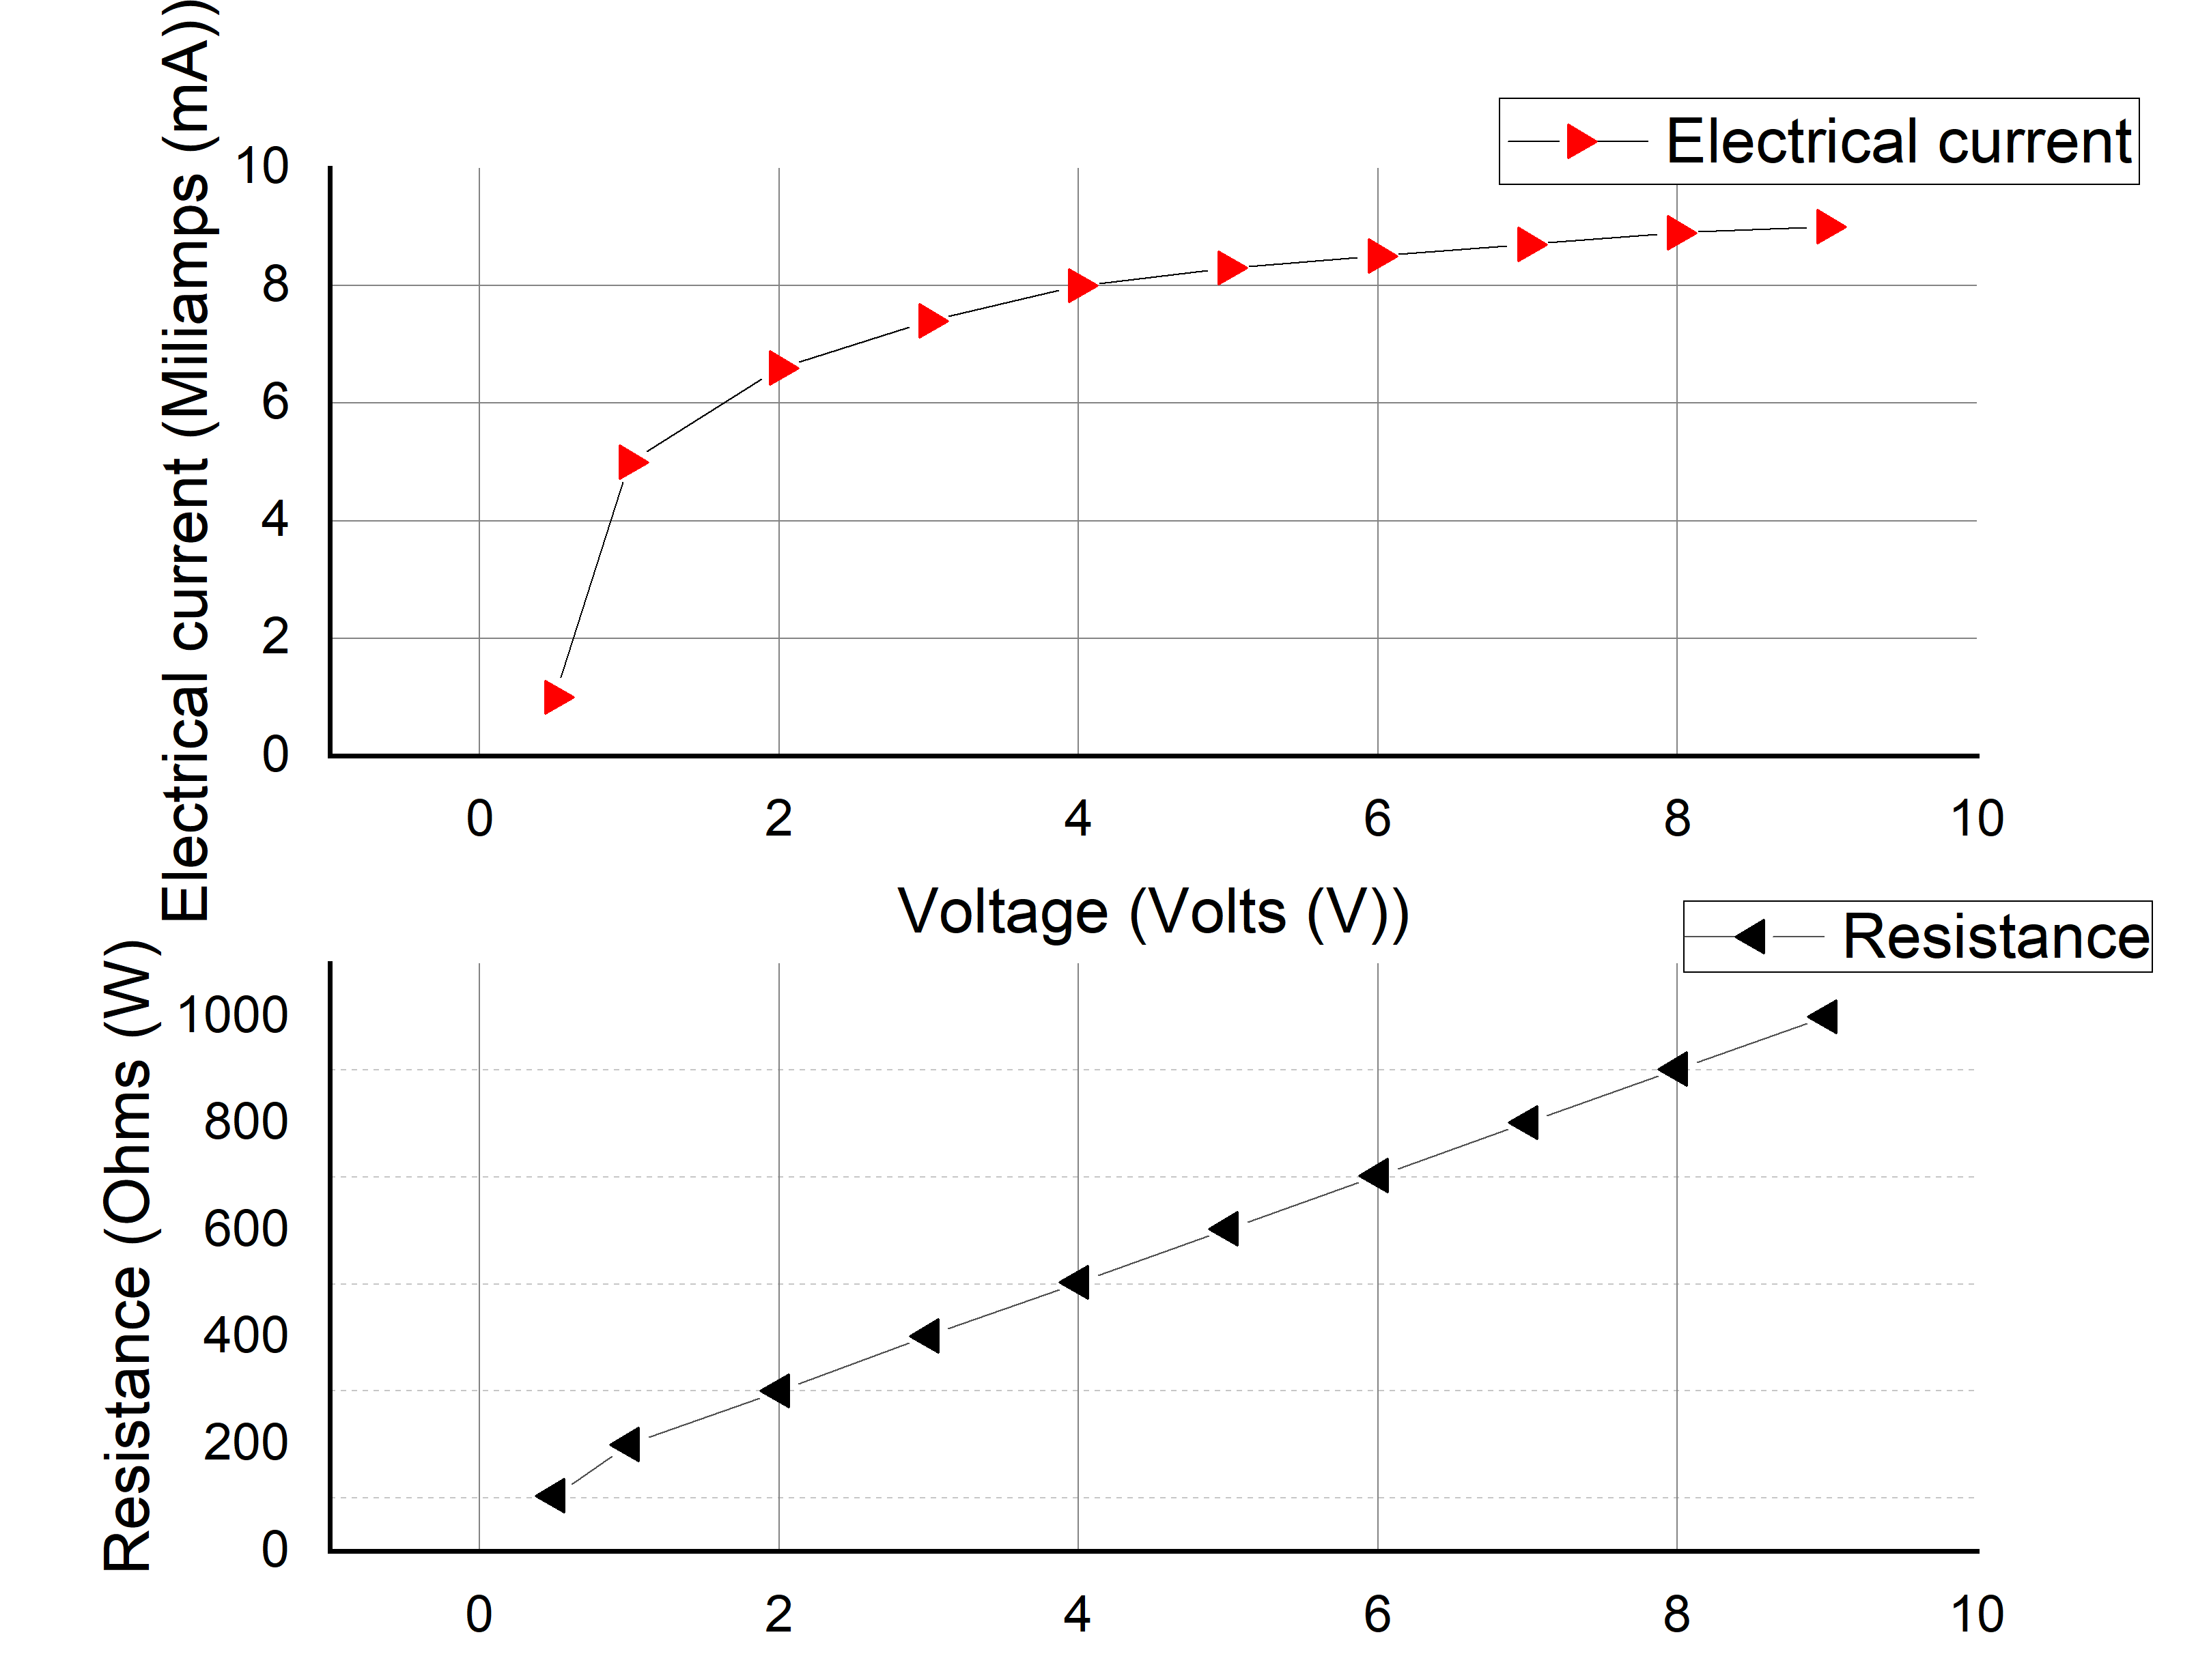
\includegraphics[scale=0.3]{Images/Graph1.png}
      \textcolor{MiColor2}{\textbf{Gráfica 1: Mediciones del voltaje ($V$) de diferentes cargas eléctricas.}}
\end{center}

\begin{center}
   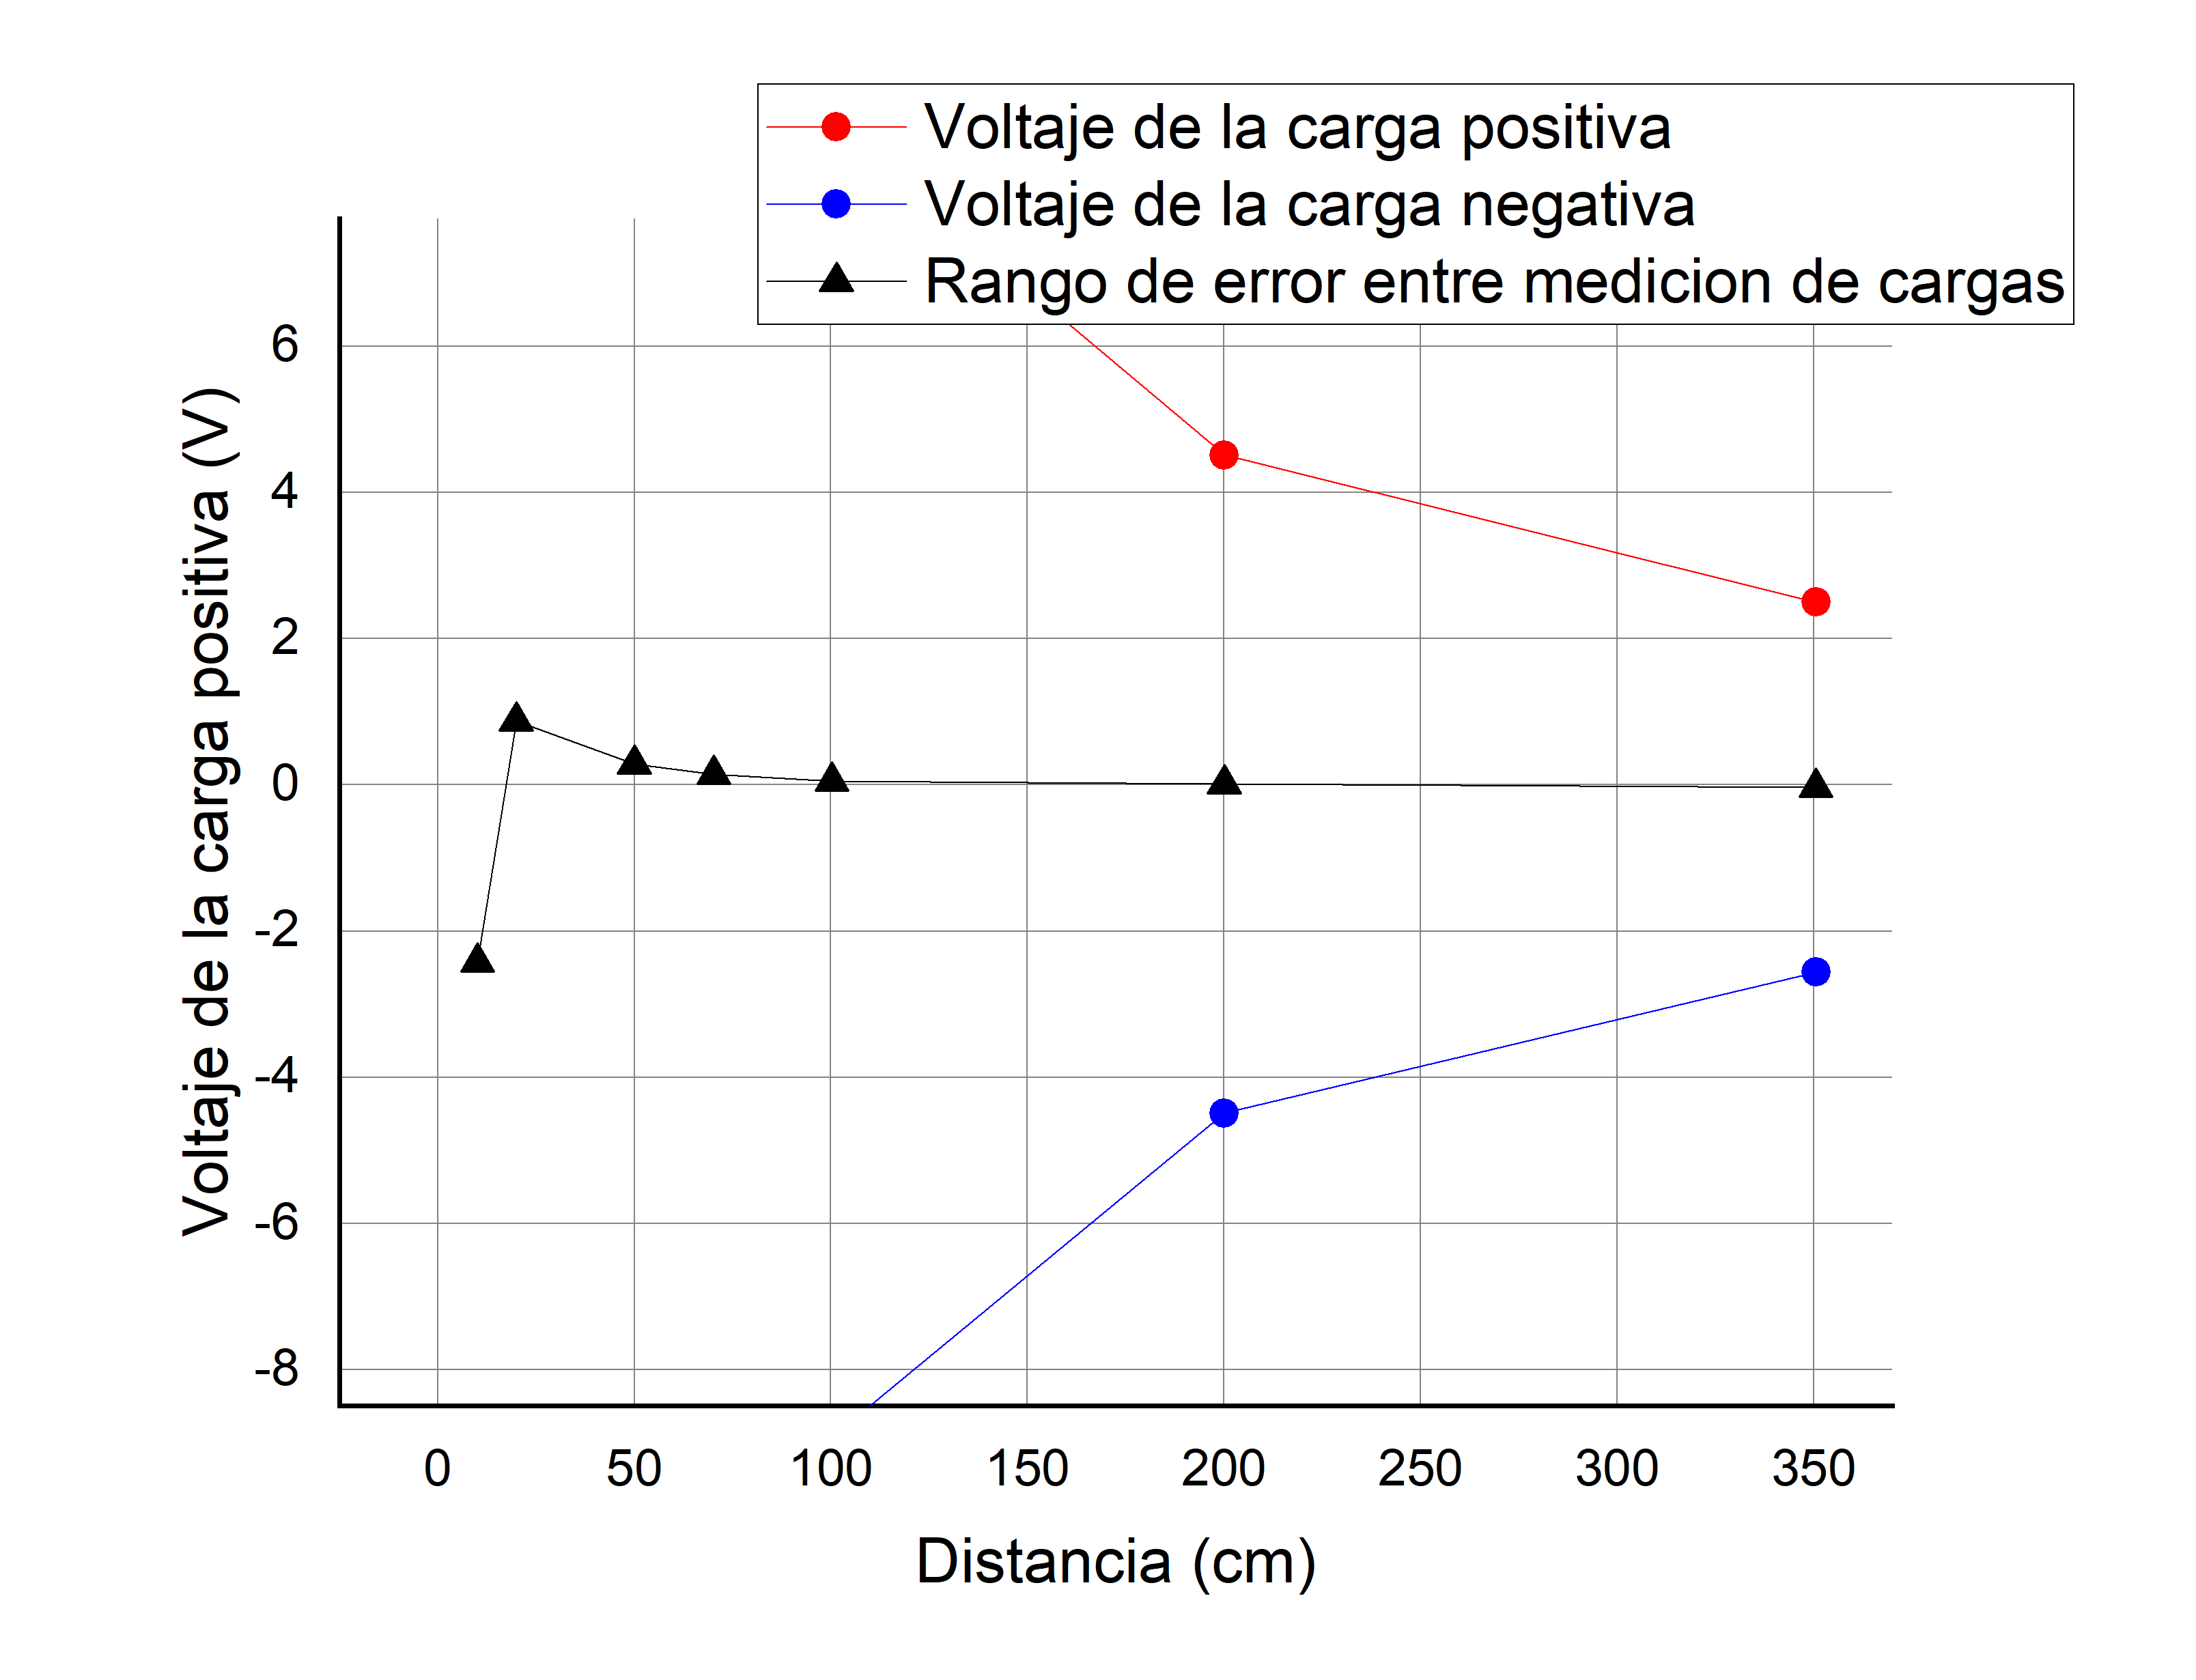
\includegraphics[scale=0.3]{Images/Graph2.png}
    \textcolor{MiColor2}{\textbf{Gráfica 2: Error de mediciones de diferentes cargas eléctricas.}}
\end{center}

\begin{center}
    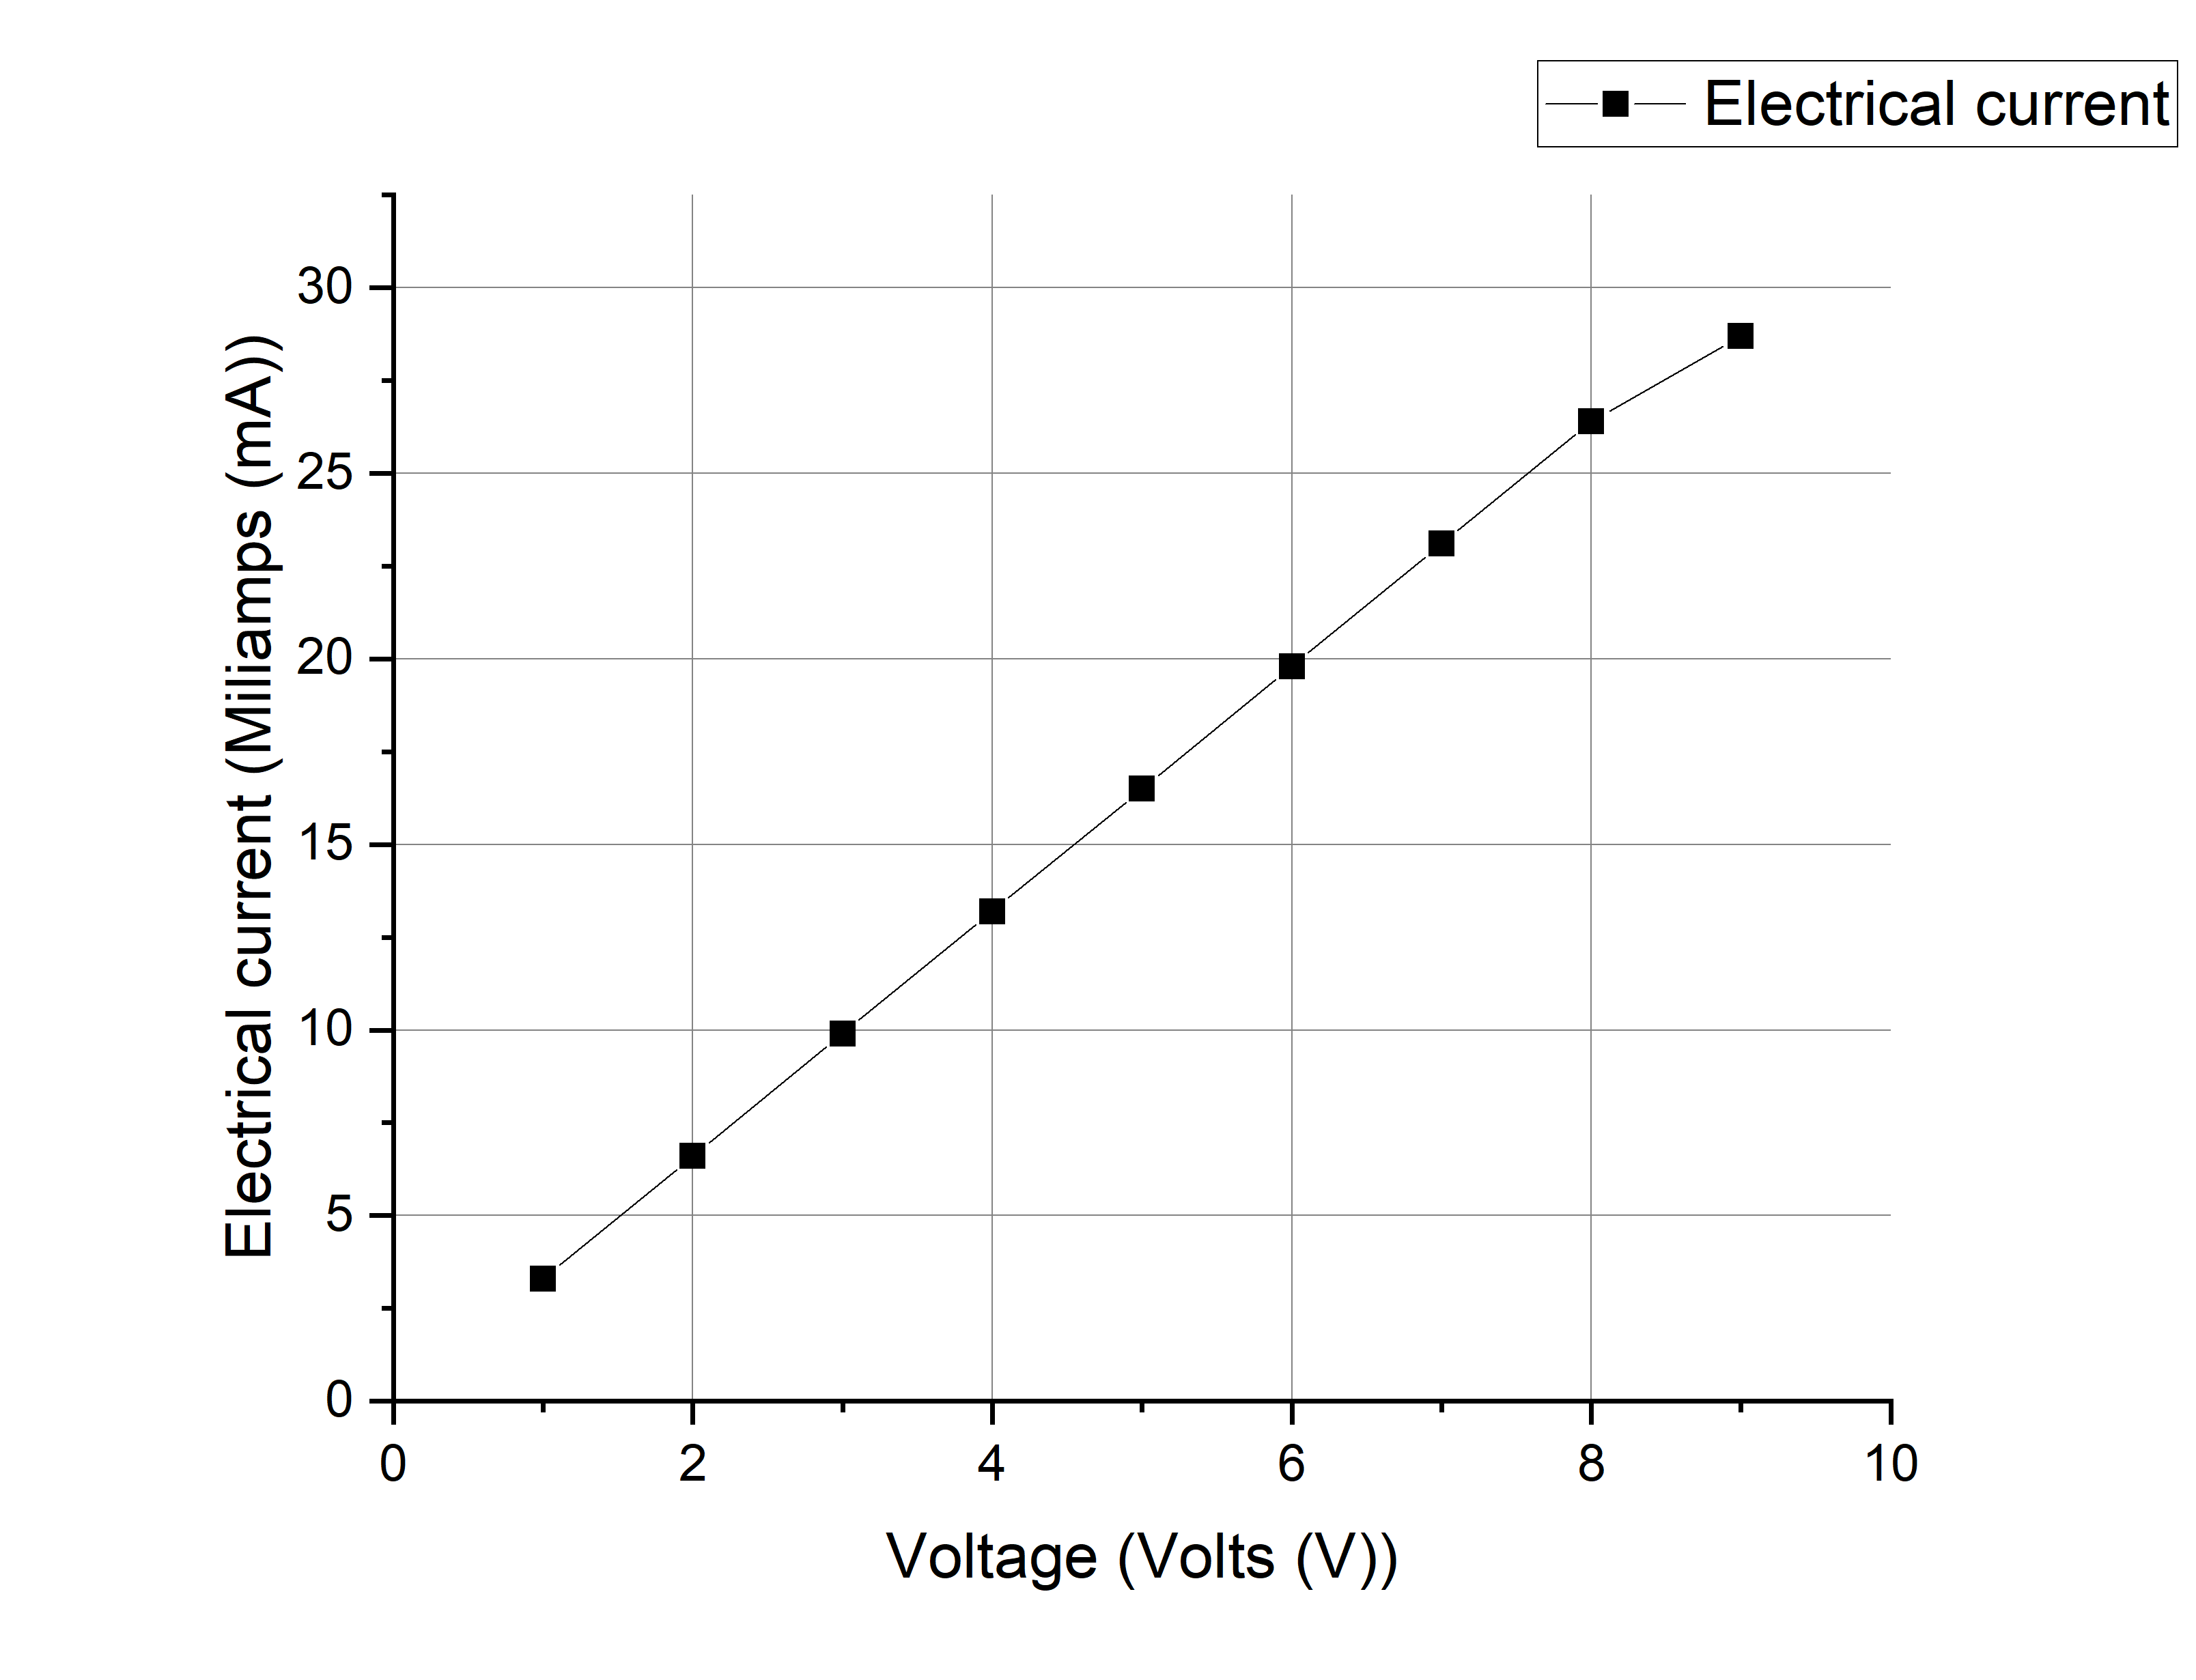
\includegraphics[scale=0.3]{Images/Graph3.png}
    \textcolor{MiColor2}{\textbf{Gráfica 3: Comparación y relación del campo eléctrico con el equipotencial para una sola carga positiva.}}
\end{center}

\begin{center}
    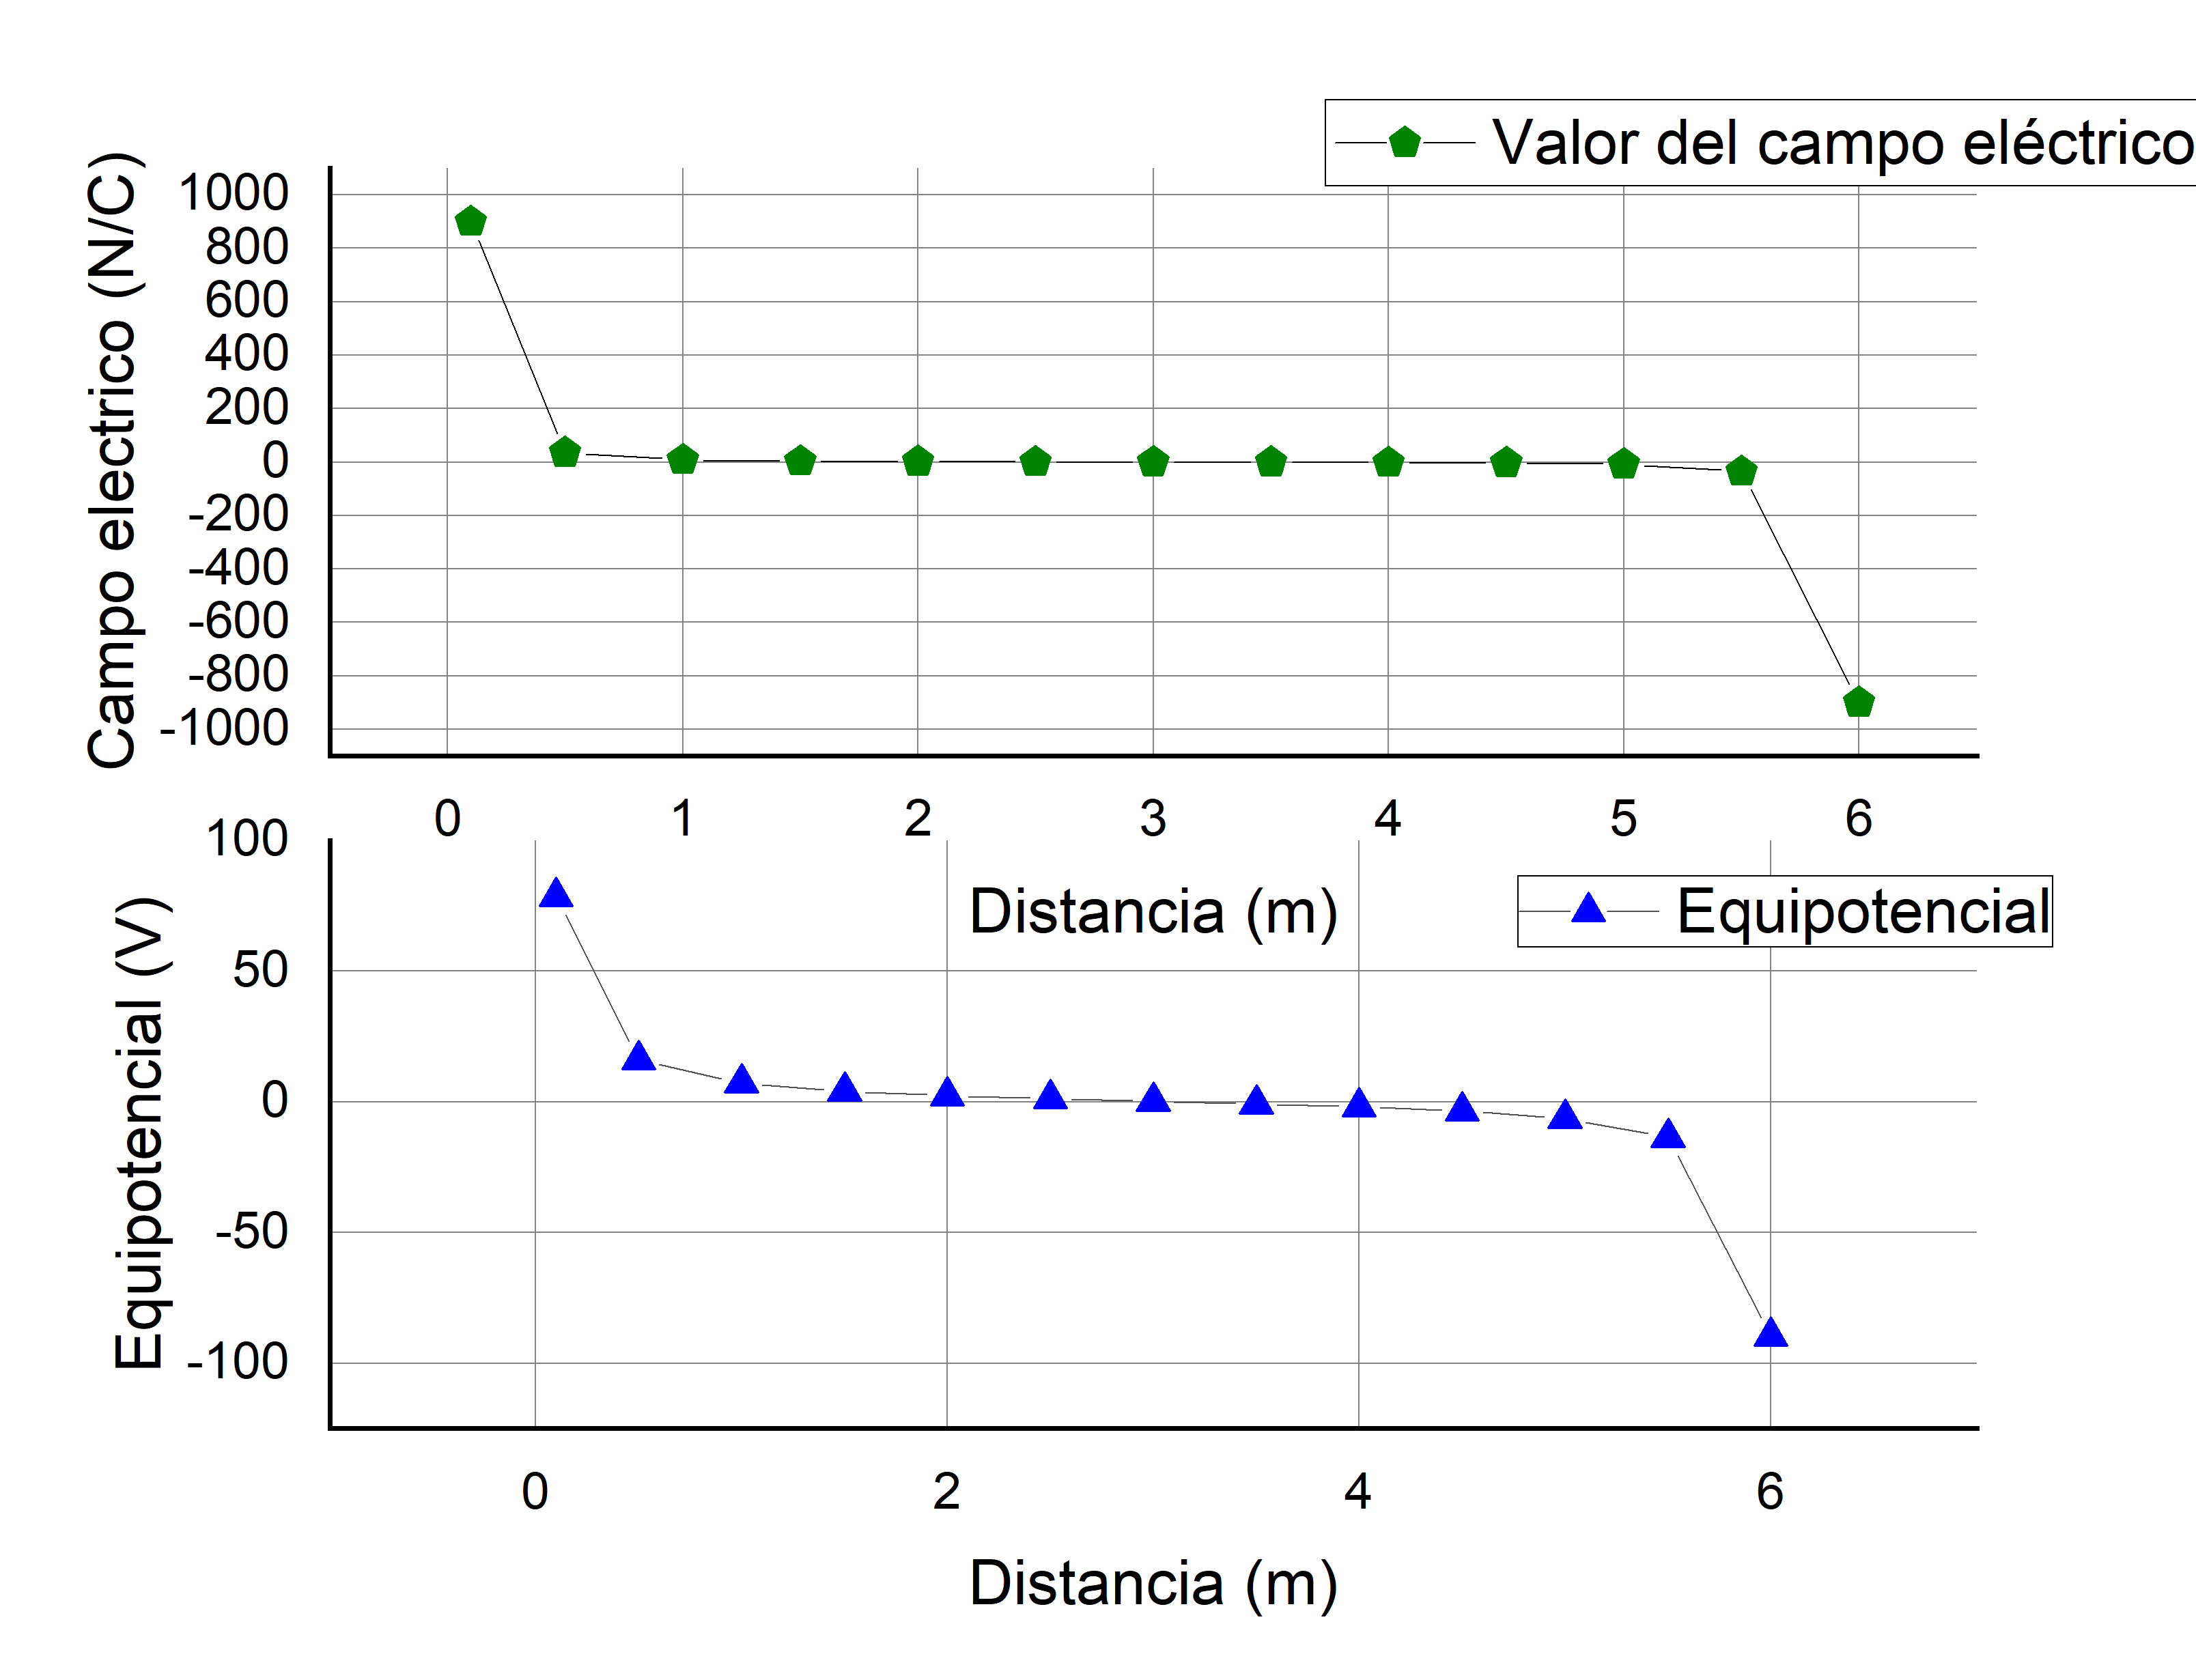
\includegraphics[scale=0.3]{Images/graph4.png}
    \textcolor{MiColor2}{\textbf{Gráfica 4: Comparación y relación del campo eléctrico con el equipotencial para dos cargas de signo opuesto.}}
\end{center}

\begin{center}
   \href{https://www.youtube.com/watch?v=dQw4w9WgXcQ}{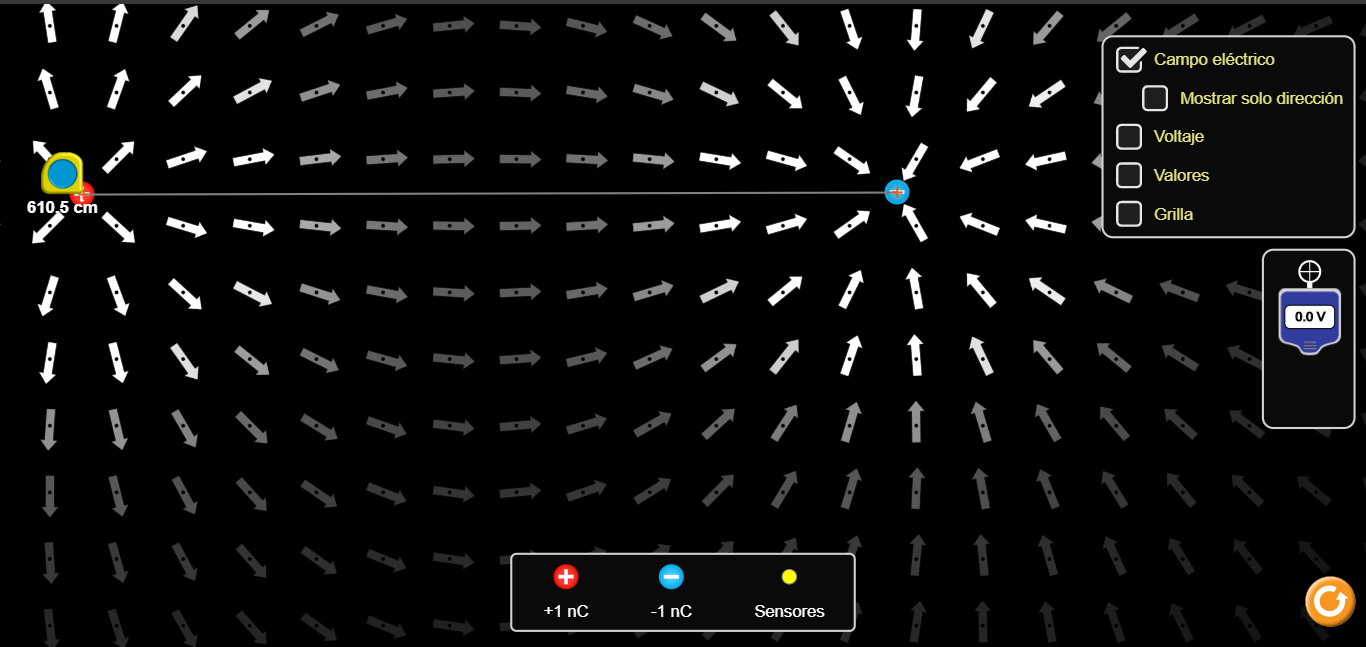
\includegraphics[scale=0.23]{Images/Captura1.PNG}}
    \textcolor{MiColor2}{\textbf{Captura 1: Bajo esta premisa fue como se calculo la gráfica 4.}}
\end{center}

\begin{center}
    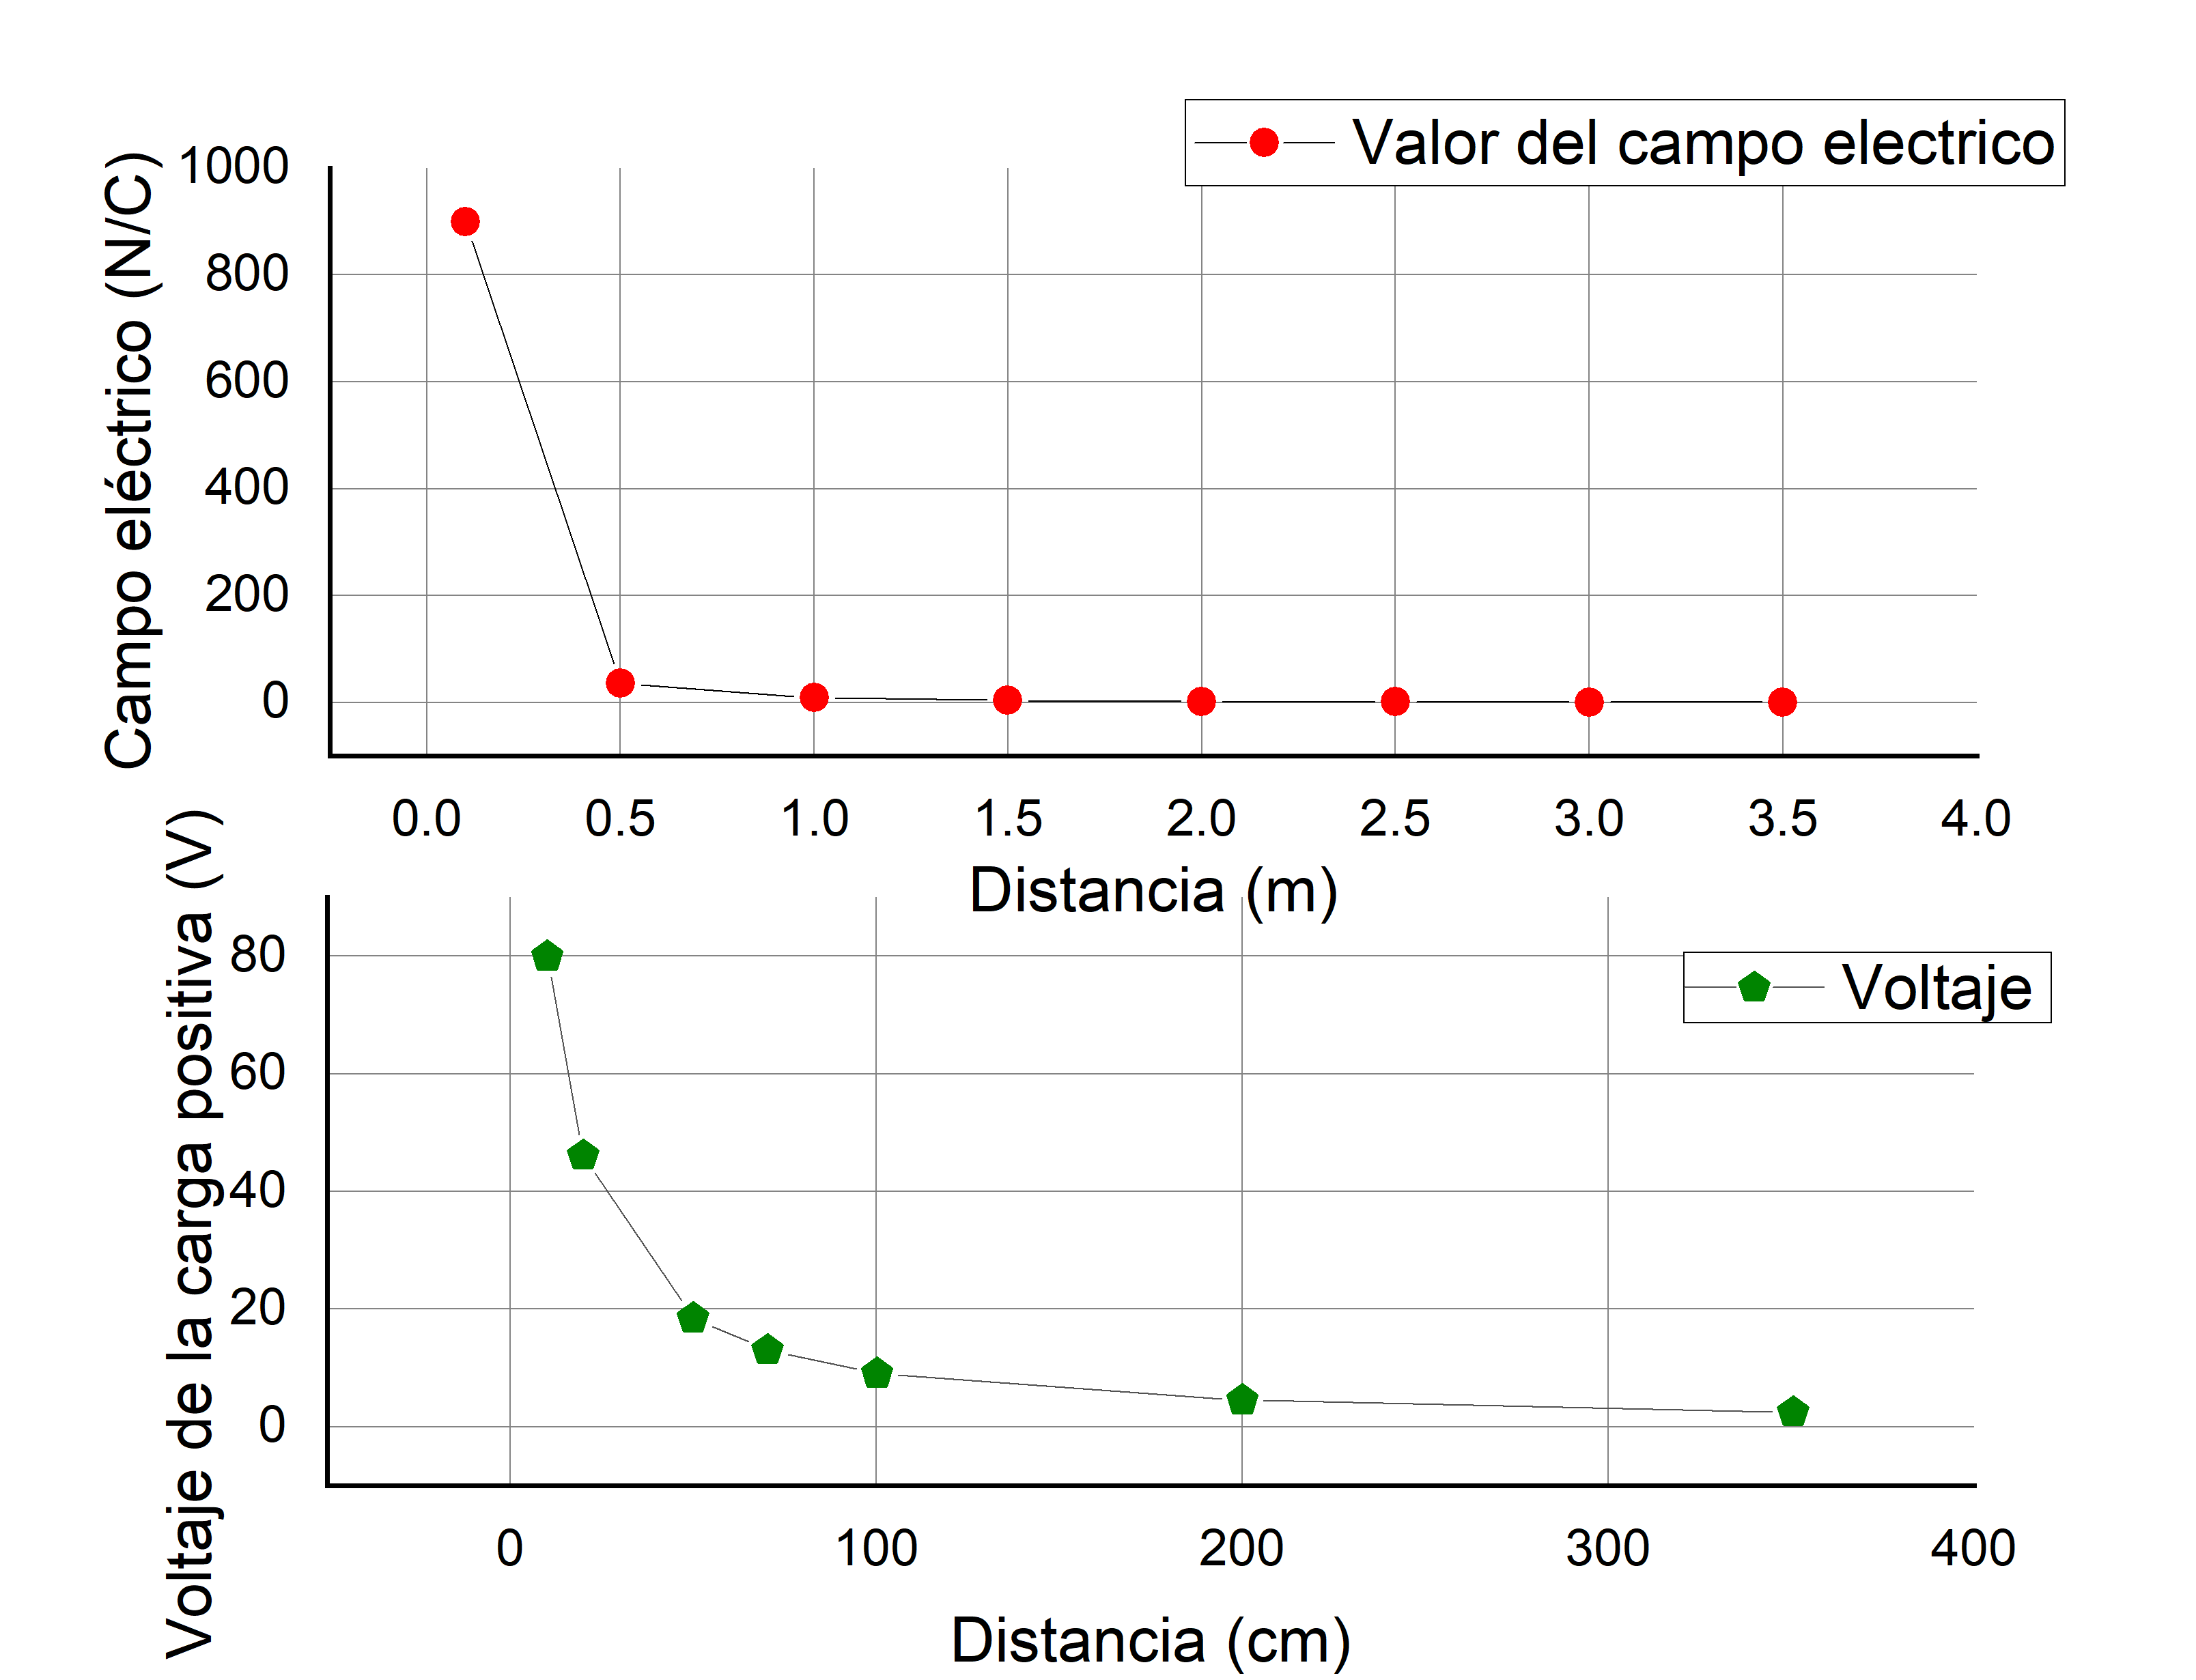
\includegraphics[scale=0.3]{Images/graph5.png}
    \textcolor{MiColor2}{\textbf{Gráfica 5: Corporación y relación del campo eléctrico y de la carga eléctrica de una carga positiva.}}
\end{center}
\section{\textcolor{MiColor1}{\textbf{Discusión}}}
En primera instancia se puede observar en la Gráfica 1 de Mediciones del voltaje ($V$) de diferentes cargas eléctricas, un decaimiento en el voltaje de forma cuadrática en ambos casos, si aplicamos un valor absoluto al comportamiento del voltaje para la carga negativa, se aprecia una simetría con respecto al eje de la distancia al rededor de los $0 cm$, lo cual tiene sentido pues las cargas en cuestión son opuestas en magnitud. Si se observa la gráfica síguete (Gráfica 2: Error de mediciones de diferentes cargas eléctricas) Se observa que bajo los $10 cm$ de medición el error de medición es considerablemente mayor comparación de los $10 cm$ en adelante mostrando una desviación de $\pm{2.3 V}$  otorgándonos un porcentaje de error del $\%2.43$ disminuyendo casi linealmente hasta los $50cm$. Esto debido a que el error erradica en la precisión del cursor y el indicador del equipotencial. \par
Siguiendo con las gráficas comparativas entre el potencial eléctrico ($N/C$) y el equipotencial ($V$), se puede apreciar un comportamiento muy similar con decaimiento cuadráticocomo, la expresión de la ley de Coulomb que está presente en la expresión de campo eléctrico, dictan. concordando de misma forma con la Gráfica 5(Corporación y relación del campo eléctrico y de la carga eléctrica de una carga positiva) en donde se observa  el mismo comportamiento consistente el calculo de las magnitudes con respecto a una distancia creciente. Por último se analiza la Gráfica 4: Comparación y relación del campo eléctrico con el equipotencial para dos cargas de signo opuesto. Donde conforme evoluciona la distancia en el que el equipotencial se encuentra, ya que las cargas están alejadas a una distancia considerablemente grande, la gráfica se aplana hasta el equilibro a una distancia igual entre las cargas. Comportándose de misma forma hacia la carga negativa. 
\section{\textcolor{MiColor1}{\textbf{Conclusiones}}}
Durante el presente documento, se han mostrado algunos sistemas electromagnéticos simples para el análisis de los conceptos más básicos que involucran estos fenómenos mediante el método de comparación de gráficas y el contraste de ellas con la teoría matemática que rodea a cada concepto. Ya que se puede estudiar esta área de la física como fenómenos ondulatorios, es claro que la disminución del campo eléctrico en el espacio tridimensional sigue la ley de la inversa del cuadrado. El trabajar con la simulación en el software phet brindó un buen entendimiento de lo que ocurrió físicamente y profundamente se comprendió la teoría matemática al contrastar los resultados cuales fueron  buenos y precisos. 
\section{\textcolor{MiColor1}{\textbf{Agradecimientos}}}
Agradecemos al doctor Mario Pérez González por brindarnos apoyo escolar para realizar esta practica y conocimiento para utilizar el software OriginPro, igualmente agradecemos a todos los doctores y expertos de la Universidad de Colorado Boulder, pues gracias a ellos se tuvo acceso al software \textit{PhET}.
\begin{thebibliography}{0}
\bibitem{1}\textcolor{MiColor2}{\protect\href{http://www.labvirfis.com/textos/serway1.pdf}{ R.A. Serway, J.W. Jewett Jr., Física para Ciencias e Ingeniería con Física Moderna, séptima edición, Cengage Learning, México, 2009.}} \par
\bibitem{2}\textcolor{MiColor2}{\protect\href{https://www.u-cursos.cl/usuario/42103e5ee2ce7442a3921d69b0200c93/mi_blog/r/Fisica_General_-_Fisica_Universitaria_Vol_2__ed_12\%28Sears-Zemansky\%29.pdf}{H.D. Young, Y. Freedman, Física Universitaria con Física Moderna, décimo tercera edición, PEARSON, México, 2013.}} \par
\bibitem{3}\textcolor{MiColor2}{\protect\href{http://www.irya.unam.mx/~g.bruzual/Mecanica_Clasica/Analisis\%20Vectorial\%20-\%20R.\%20Spiegel,\%20S.\%20Lipschutz.pdf}{M.R. Spiegel, S. Lipschutz, D. Spellman, Análisis Vectorial, segunda edición, McGrawHill Educación, México, 2009.}} \par
\bibitem{4}\textcolor{MiColor2}{\protect\href{http://www.fulviofrisone.com/attachments/article/485/Resnick-Fisica\%20Vol\%202.pdf}{D. Halliday, R. Resnick, \& K.S. Krane, Física Volumen 2, cuarta edición, Editorial Continental, México, 1999.}} \par
\bibitem{5}\textcolor{MiColor2}{\protect\href{https://phet.colorado.edu/sims/html/charges-and-fields/latest/charges-and-fields_es.html}{Charges and Fields 1.0.47. PhET: Interactive Simulations. \\ https://phet.colorado.edu/sims/html/charges-and-fields/latest/charges-and-fields\_es.html. \\ 2020 (Accessed 21 August 2020)}} \par
\bibitem{6}\textcolor{MiColor2}{\protect\href{https://www.raco.cat/index.php/Ensenanza/article/view/83239/108222}{Furió-Mas, Carles, and Jenaro Guisasola Aranzabal. "Dificultades de aprendizaje de los conceptos de carga y de campo eléctrico en estudiantes de bachillerato y universidad." Enseñanza de las ciencias: revista de investigación y experiencias didácticas 16.1 (1998): 131-146.}} \par
\bibitem{7}\textcolor{Black}{J. Wilson, A.J. Bufa \& B. Lou, Física, Sexta edición, PEARSON, México, 2007.} \par
\bibitem{8}\textcolor{MiColor2}{\protect\href{http://esystems.mx/BPC/llyfrgell/0296.pdf}{D. Giancoli, Física para Ciencias e Ingenierías. Volumen 2, Cuarta edición, PEARSON, México, 2009}}
\bibitem{9}\textcolor{Black}{Stanley V. Marshall, Richard E. DuBroff and Gabriel G. Skitek, Electromagnetismo. Conceptos y Aplicaciones, Cuarta Edición, México, 1997.} \par
\bibitem{10}\textcolor{MiColor2}{\protect\href{https://repositoriodigital.ipn.mx/bitstream/123456789/10744/1/25_LAJPE_285_Manuel_Sandoval.pdf}{Sandoval, M., and César Mora. "Modelos erróneos sobre la comprensión del campo eléctrico en estudiantes universitarios." (2013).}}

\end{thebibliography}

\end{multicols}

\end{document}
